\documentclass [11pt, twoside]{article}

%\usepackage{times}
\usepackage{graphicx}
\usepackage{ifthen}
\usepackage{xspace}
\usepackage{fancyhdr}
\usepackage{moreverb}
%\usepackage{hyperref}
\usepackage{float} % for the [H] 
\usepackage{amsmath}

% solution switch
\newboolean{showsolution}
\setboolean{showsolution}{false}


%layout
\topmargin      -5.0mm
\oddsidemargin  6.0mm
\evensidemargin -6.0mm
\textheight 215.5mm
\textwidth      160.0mm
\parindent        1.0em
\headsep          10.3mm
\headheight        12pt
\lineskip    1pt
\normallineskip     1pt

%header
\lhead{Programming Languages \\ 2021}

\rhead{Prof. O. Nierstrasz\\
Mohammadreza Hazhirpasand, Joel Niklaus}
\lfoot{page \thepage}
\rfoot{\today}
\cfoot{}

\renewcommand{\headrulewidth}{0.1pt}
\renewcommand{\footrulewidth}{0.1pt}

\renewcommand{\thesubsection}{\arabic{subsection}}

%enumeration
\newenvironment{myitemize}{%
     \begin{itemize}
     \setlength{\itemsep}{0cm}}
     {\end{itemize}}

\newenvironment{myenumerate}{%
     \begin{enumerate} \setlength{\itemsep}{0cm}}
     {\end{enumerate}}


%solution
\ifthenelse{\boolean{showsolution}}
   {  \newcommand{\solution}[1]{
   	\noindent\underline{\textbf{Answer:}}\\[2mm]
   	 \textsl{#1}
	 \vspace{10pt}
	 \normalsize
	}
  }
  {  \newcommand{\solution}[1]{} }

\newcounter{exnum}
\def\xexercise{\fontsize{12}{10}\fontseries{bx}\selectfont}
\def\xnormal{\fontseries{m}\fontshape{n}\selectfont}


\newcommand{\exercise}[1]{%
     {\addtocounter{exnum}{1}\vskip 0.8cm{\xexercise \noindent Exercise
\arabic{exnum} (#1)} \xnormal} \vskip 0.3cm} 
 \newcommand{\aufgabe}[1]{
     {\addtocounter{exnum}{1}\vskip 0.8cm{\xexercise \noindent Aufgabe
\arabic{exnum} (#1)} \xnormal} \vskip 0.3cm} 

\pagestyle{fancy}


% ===============ABBREVIATIONS==============================
\newcommand{\eg}{\emph{e.g.,}\xspace}
\newcommand{\ie}{\emph{i.e.,}\xspace}
\newcommand{\etc}{\emph{etc.}\xspace}


\begin{document}

% title
\section*{\ifthenelse{\boolean{showsolution}}{Solution }{}\xspace{}Serie 2 - Postscript}

% - - - - - - - - - - - - - - - - - - - - - - - - - - - - - - - - - - - - - -
\subsection*{Exercise 1}
Answer the following questions about Postscript:

\begin{myitemize}

\item How do you manipulate the coordinate system? 
\solution{There are three standard operators to manipulate it, namely
translate, scale and rotate. You can even define your own transformation using
the operator concat.}

\item Why would you define your own dictionaries? 
\solution{Dictionaries can be reused, and should help to avoid code
duplication. A pretty good example are the arrows on lecture slide 2.34. - You
can define your own local variables, without having to fear the names have
been used elsewhere.}

\item When should you use \texttt{translate} instead of \texttt{moveto}?
\solution{Translate should be used in conjunction with relative coordinates.
For example, if you define a function which should draw an object starting at
the center of the page (and not at the origin), you should use translate in
order to move the origin to the center. Then the object is drawn relative to
the new coordinate system.}

\item When would you use a matrix instead of \texttt{gsave}/\texttt{grestore}?


\item Why is it important to leave the stack in a consistent state?


\item Implement the equivalent of the following piece of code in postscript:
\begin{verbatim}
public int f(int a, int b) {
    int d = x(a, b);
    z(a, b);
    return d;
}

public int x(int a, int b) {
    return a - b;
}

public int z(int a, int b) {
    return a + b;
}
\end{verbatim}



%\solution{\texttt{gsave} saves the current graphical state}
%\item How could you use dictionaries to simulate object-oriented programming?
%(Give a brief explanation, you don't need to provide any implementation of
%your answer) \solution{}

\end{myitemize}

% - - - - - - - - - - - - - - - - - - - - - - - - - - - - - - - - - - - - - - - - - - - - - - - - - - - - - - - - - - - - - - - - - - -
\subsection*{Exercise 2}
Write the procedures to get the following drawings:
\vspace{10pt}

\begin{figure}[htbp]
\begin{center}
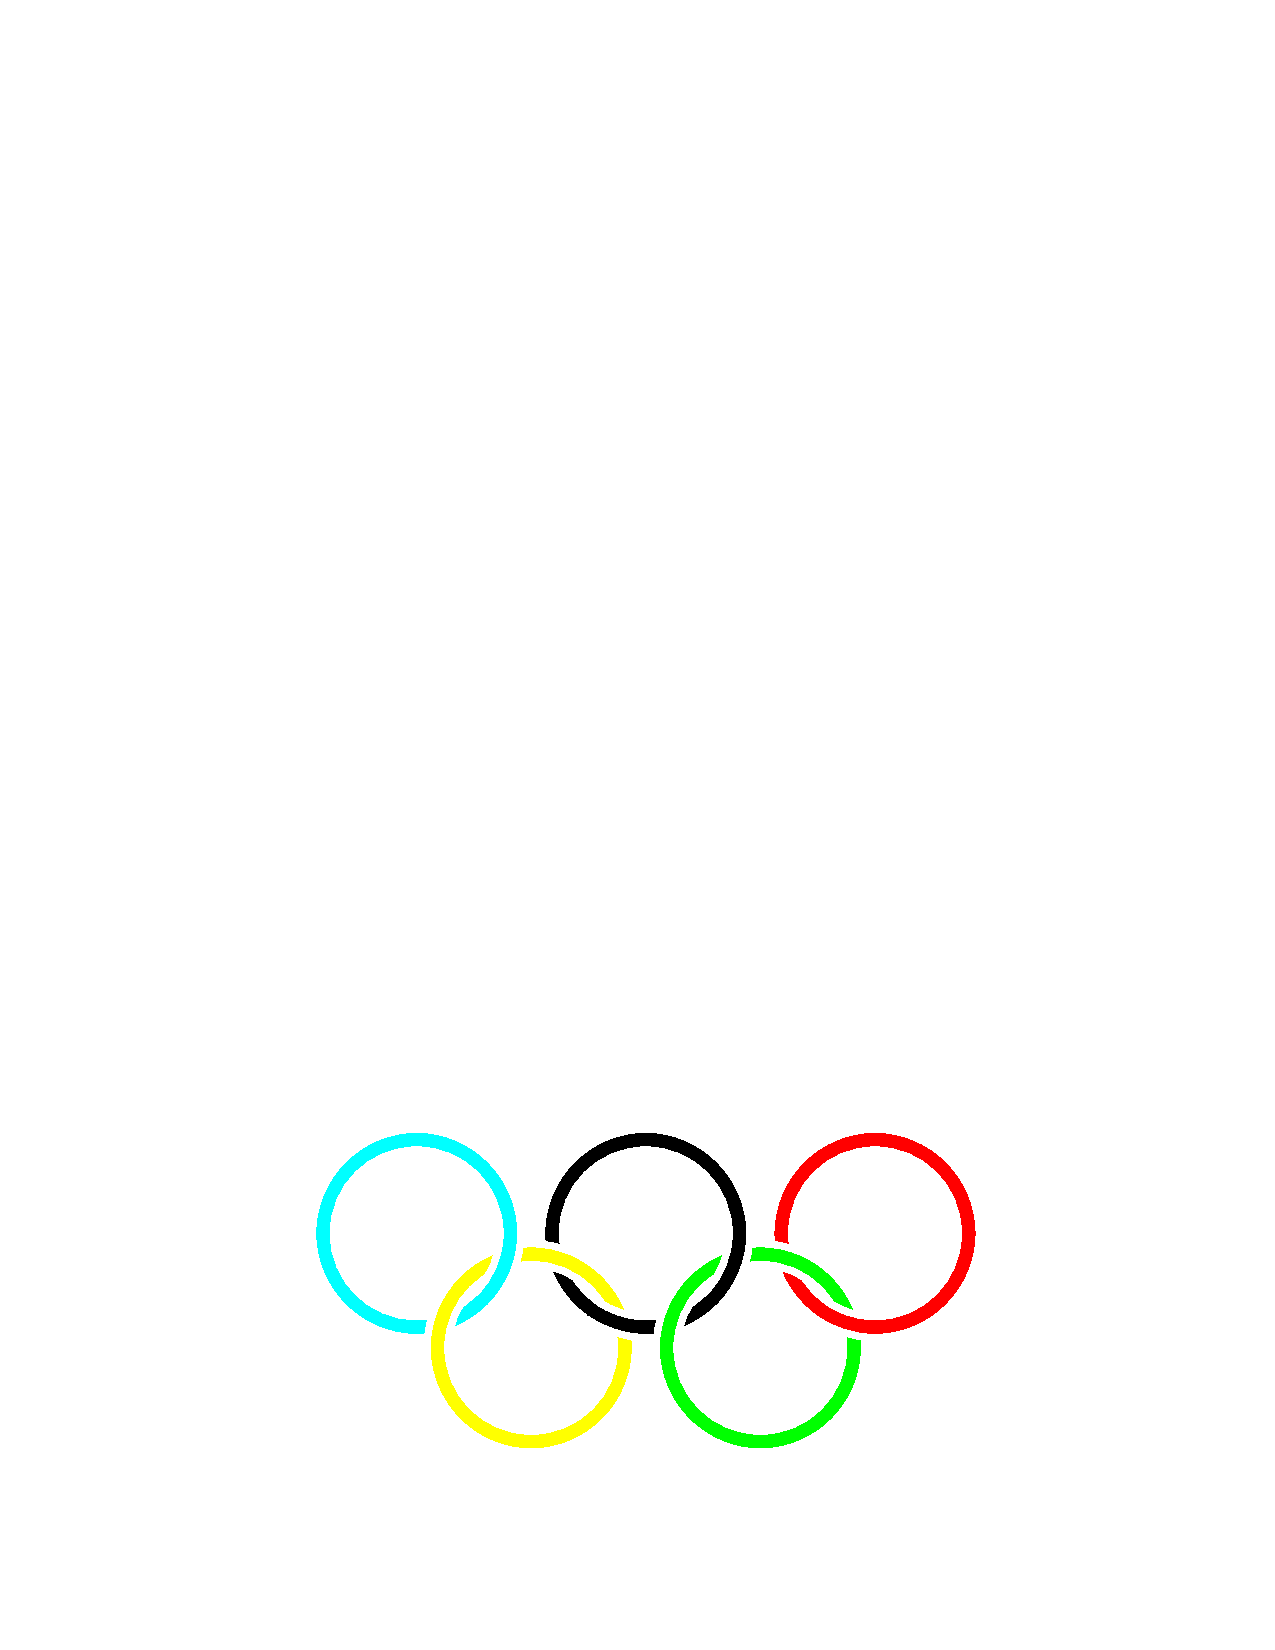
\includegraphics[scale=0.5]{source/olympicCircles.pdf}
\caption{Olympic circles}
\label{default}
\end{center}
\end{figure}



\textbf{Hints:} To make the circles cross one another you should paint the circles then redraw the small arc that is foreground

\solution{\input{source/olympicCircles.ps}}

% - - - - - - - - - - - - - - - - - - - - - - - - - - - - - - - - - - - - - - - - - - - - - - - - - - - - - - - - - - - - - - - - - - -
\subsection*{Exercise 3}
Write the procedures to get the following drawings:\\
\begin{figure}[H]
    \centerline{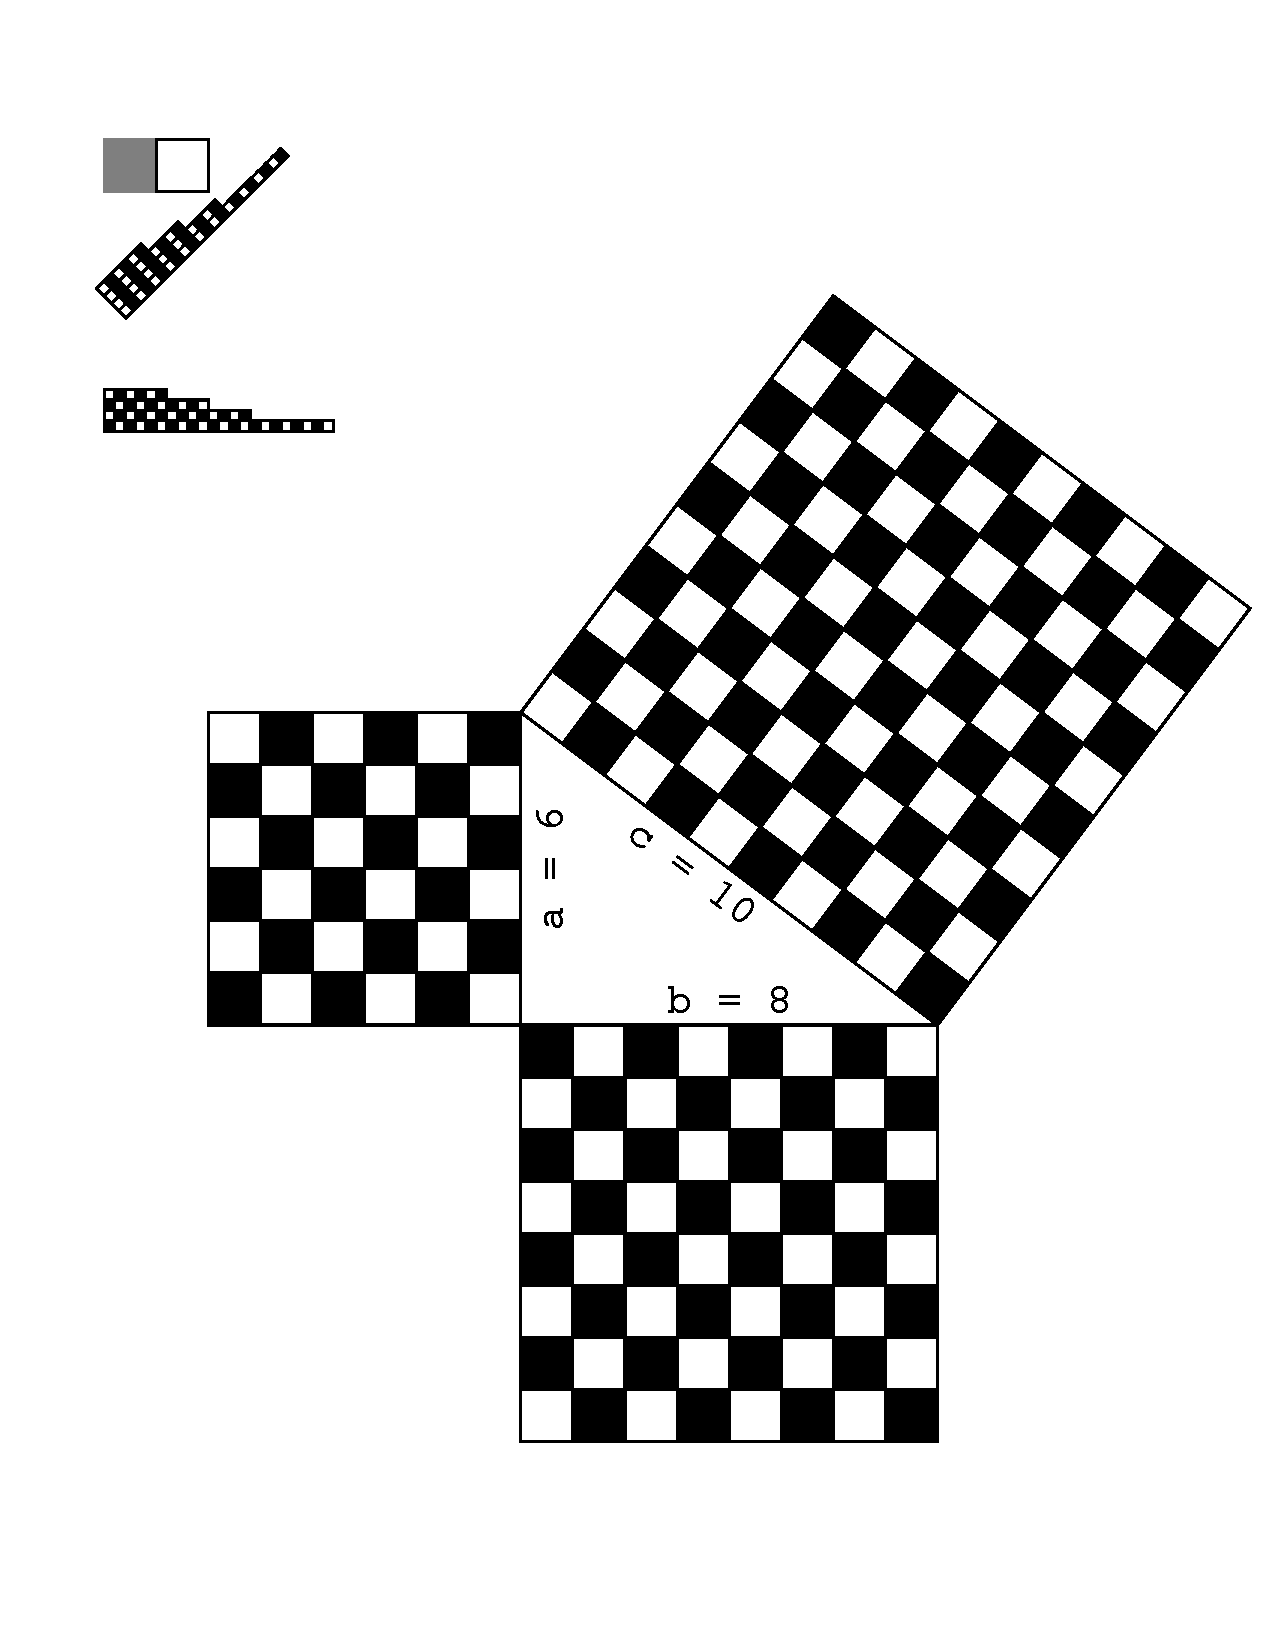
\includegraphics[height=10cm]{exercise3}}
\end{figure}	



The exercises consist of the following steps:
\begin{enumerate}
	\item Create a procedure \texttt{/box} drawing a rectangle of a given size
	\item Create a procedure \texttt{/filledbox} and \texttt{/borderedbox}
		both drawing a rectangle, one completely filled, the other only with
		outline drawn. Both procedures expect a gray color and a size.
	\item Create a procedure \texttt{/drawline} drawing a line of alternating
		filled and bordered rectangles. It expects the size of each rectangle
		and the number of rectangle pairs as arguments.
	\item Create the procedures \texttt{/evenline} and \texttt{/oddline} both
		working similar to \texttt{/drawline} but one starting with a filled
		rectangle and the other with a outlined rectangle. Both take the same
		arguments as \texttt{/drawline}
	\item Create a procedure \texttt{/chessboard} drawing vertically alternating
		\texttt{/evenline} and \texttt{/oddline}. The output should be a
		rectangular chessboard. It takes the number of pairs of even/oddlines
		and the size of a single rectangle as argument. 
\end{enumerate}


\solution{\fontsize{8pt}{10pt}
\begin{verbatim}
% --------------------------------------------------
% Squares
% --------------------------------------------------
/inch {72 mul} def
/centersquare
  { newpath
    .5 .5 moveto
    -.5 .5 lineto
    -.5 -.5 lineto
    .5 -.5 lineto
   closepath
  } def

  2.5 inch 6 inch translate
  1 16 div setlinewidth
  1 1 5 
  { gsave
      .5 mul inch dup scale
      centersquare
      stroke
    grestore
  } for
showpage

% --------------------------------------------------
% Rotation
% --------------------------------------------------
/Times-Roman findfont
10 scalefont
setfont
300 500 translate
0 10 540 {              % go from 0 to 540 degrees in 10 degree steps
  gsave                 % keep rotations temporary
    dup rotate          % rotate by degrees on stack from 'for'
    8 div 0 moveto      % divide angle by 8 and use it to shift in x direction.
    (postscript) show
  grestore              % get back the unrotated state

} for                   % iterate over angles
showpage
\end{verbatim}}

% - - - - - - - - - - - - - - - - - - - - - - - - - - - - - - - - - - - - - - 


\end{document}









